% Copyright 2024 Kieran W Harvie. All rights reserved.

\section{Incidence Algebra}
While working on the harmonic series I got an itch to revise some incidence algebra.
This is because of the use of the inclusion-exclusion principle,
which is beautifully generalized by the structure. 

\subsection{Poset Revision}
A poset $P$ is set with an operator $\preceq$ referred to as the `partial order' and works as one would expect, meaning for $x,y,z\in P$ :
\begin{itemize}
	\item {\bf Reflexivity:}  $x\preceq x$.
	\item {\bf Antisymmetry:}  If $x\preceq y$ and $y\preceq x$ then $x=y$.
	\item {\bf Transitivity:}  If $x\preceq y$ and $y\preceq z$ then $x\preceq z$.
\end{itemize}
We write $x\prec y$ is $x\preceq$ and $x\neq y$ and a chain is a subset of $P$ such that:
\[x_0\prec x_1 \prec x_2 \prec \dots \prec x_n\]
A multichain is a subset of $P$ such that:
\[x_0\preceq x_1 \preceq x_2 \preceq \dots \preceq x_n\]
A closed interval $[x,y]$ is a subset of $P$ defined as:
\[[x,y] = \{z\,:\,x\preceq z\preceq y \text{ where }x,y,z\in P\}\]
The set of all intervals of a $P$ is denoted $\operatorname{Int}(P)$ and a locally finite poset $P$ is one where each closed interval is finite.

\subsection{Incidence Algebra Definition}
The Incidence Algebra of $P$ over $K$ is denoted $I(P,K)$ where the vector space is the space of functions $K^{\operatorname{Int}(P)}$ with addition and scalar multiplication defined in the normal way.
The bilinear function of the algebra is called convolution and is defined as:
\[(f*g)([x,y]) = \sum_{z\in [x,y]}f([x,z])g([z,y])\]
Where meaning is obvious a lot of symbols are dropped:
\[fg[x,y] = \sum_{z\in [x,y]}f[x,z]g[z,y]\]
Some special names elements are the delta and zeta functions:
\[\zeta[x,y] = 1,\quad\delta[x,y] = \begin{cases}1&x=y\\0&x\neq y\end{cases}\]
These functions are defined their useful convolution properties:
\begin{equation*}
\begin{aligned}
	f\zeta[x,y] =& \sum_{z\in [x,y]}f[x,z]\\
	\zeta f[x,y] =& \sum_{z\in [x,y]}f[z,y]\\
	f\delta[x,y] =& \delta f[x,y] = f[x,y]\\
\end{aligned}
\end{equation*}
We can see that the set of invertible functions $K^{\operatorname{Int}(P)}$ are a group with unit element $\delta$.
To this end  with define a new function $\mu$ called the Möbius function:
\[\mu[x,y] = \begin{cases}1&x=y\\-\sum_{x\preceq z\prec y}\mu(x,z)&x\prec y\\0&y\prec x\\\end{cases}\]
You can show that:
\[\mu\zeta = \delta\]
An important use for this group is as a group action from this group onto $K^P$ such that:
\[(f\cdot a)(x) = \sum_{y\preceq x}f(y)a[y,x]\]

\subsection{General Inclusion-Exclusion Principle}
Assume all the previous results are true\footnote{Prove them yourself.} we get the following corollary.
Let $f,g\in K^P$ then:
\[g(x) = (f\cdot \zeta)(x) \Leftrightarrow f(x) = (g\cdot \mu)(x)\]
Or more verbosely:
\[g(x) = \sum_{y\preceq x}f(y) \Leftrightarrow f(x) = \sum_{y\preceq x}g(y)\mu[y,x]\]
For a sketch of how this is generalization of the more common inclusion-exclusion principle consider the following:
\begin{enumerate}
	\item Let $(A_i)_{i\in I}$ be a family of sets indexed by $I$ and let $P$ be the poset of subsets of $I$ ordered by inclusion.
	This makes $\mu[S,T] = (-1)^{T/S}$
	\item Define $f:P\rightarrow \mathbb{N}$ where $f(T)$ is the number of elements $a$ such that:
		\[\left\{a \in \bigcup_{i\in I/T}A_i \mid i\in T \Rightarrow a\not\in A_i \right\}\]
	In natural language, this is set elements in the sets indexed by $I/T$ but not in the sets indexed by $T$.
	\item These sets are mutually exclusive so we directly get:
		\[g(T)=\begin{cases}\left|\bigcap_{i\in I/T}A_i\right| T\neq I\\\left|\bigcup_{i\in I\phantom{/I}}A_i\right|T=I\end{cases}\]
	\item $f(I)=0$ because $\bigcup_{i\in I/I}A_i = \varnothing$ applying the general inclusion-exclusion principle to $f(I)$ we get: 
		\[0=\left|\bigcup_{i\in I}A_i\right|+\sum_{T\subset I}\left|\bigcap_{i\in I/T}A_i\right|(-1)^{I/T}\quad\square\]
\end{enumerate}

\subsection{A Section Where I Drily Preform Calculations}
In this section I will preform some of the calculations I glossed over for the sketch of the common inclusion-exclusion principle proof,
all notation is inherited from there.

\subsubsection{Calculating $\mu[S,T]$:}
We will only consider the case $S\subset T$ and define $n=|T/S|$,
as other cases are given by the definition of $\mu$.
In this case $T/S$ contains at least on element and we can consider sets $X$ such that:
\[\varnothing\subseteq X\subset T/S\]
An important and immediate result is that $S$ and all $X$ are mutually exclusive as:
\[X\cup S \subset (T/S)\cup S = \varnothing\]
Hence sets $X$ such that $|(X\cup S)/S|=|X|=k$ are the $k$ elements subsets of $T/S$,
meaning there are $\binom{n}{k}$ of them.
\\

For the inductive assumption we assume for all sets $X$ such that:
\[|(S\cup X)/S| = k < n = |T/S|\]
We have:
\[\mu[S,S\cup X] = (-1)^{|(S\cup X)/S|} = (-1)^k\]
These are clearly the sets we just considered meaning we can reparametrize the following sum to get:
\begin{equation*}
\begin{aligned}
	\mu[S,T] =& -\sum_{S\subseteq X\subset T}\mu[S,X] \\
	=&-\sum_{\varnothing\subseteq X\subset T/S}\mu[S,S\cup X]\\
	=& -\left(\sum_{k=0}^{n-1}\binom{n}{k}(-1)^k\right)\\
	=& -\left(-(-1)^{n+1}+\sum_{k=0}^{n}\binom{n}{k}(-1)^k\right)\\
	=& -\left(-(-1)^{n+1}+(1-1)^n\right)\\
	=& (-1)^{n}\\
\end{aligned}
\end{equation*}
As required.

\subsubsection{Formalization of $f(T)$:}
To cleanly formalize $f(T)$ we will define a new utility function $\chi:\cup_{i\in I}A_i \rightarrow P$ such that:
\[\chi(a) = \{i\mid a\in A_i\}\]
In natural language $a$ is in the sets indexed by $\chi(a)$ and not in the sets indexed by $I/\chi(a)$,
hence $f(T)$ can be defined as:
\[f(T) = \left|\left\{a\in \bigcup_{i\in I}A_i \mid I/\chi(a)=T\right\}\right|\]
An important corollary of this formalization is:
\[T\neq T' \Rightarrow f(T)+f(T') =\left|\left\{a\in \bigcup_{i\in I}A_i \mid I/\chi(a)\in\{T,T'\}\right\}\right| \]
This follows from the underlying sets being mutually exclusive:
\[T\neq T' \Rightarrow \left\{a\in \bigcup_{i\in I}A_i \mid I/\chi(a)=T\right\}\cup\left\{a\in \bigcup_{i\in I}A_i \mid I/\chi(a)=T'\right\}=\varnothing\]
Mutual exclusivity doesn't come from any unique property of $\chi$ beyond being a function,
to see let $X$ be any set and $f$ be any function with domain $X$ and consider:
\[a\neq b\Rightarrow\{x\in X | f(x) = a\}\cup\{x\in X| f(x) = b\} = \varnothing\]
Assume $a=b$ but that the two sets do intersect then there would exist an element $x_0$ in that intersection such that:
\[a = f(x_0) = b\]
A contradiction, hence the sets are mutually exclusive.

\subsubsection{Alternative Formalization of $f(T)$:}
Although the previous formalization is enough to recover the more common inclusion-exclusion principle
there's a more standard and interesting way to write this set when $T\neq I$,
start by considering:
\[a\in\bigcap_{i\in I/T}A_i \Leftrightarrow I/T\cap \chi(a) = I/T \Leftrightarrow I/\chi(a)\subseteq T\] 
Since, by definition, for $a$ to be in the intersection of a set of sets it must be an element of each set.
(This is why $T\neq I$ as if the set of sets is empty then the statement becomes vacuous).
Likewise for an element not being in union of a set of sets we get:
\[a\not\in\bigcup_{i\in T}A_i \Leftrightarrow T\cap \chi(a) = \varnothing \Leftrightarrow I/\chi(a)\supseteq T\]
Since $a$ can't be an element of any of the $T$ sets, combining these results gives:
\[a\in\frac{\bigcap_{i\in I/T}A_i}{\bigcup_{i\in T\phantom{/T}} A_i}\Leftrightarrow I/\chi(a) = T\]
Hence:
\[\frac{\bigcap_{i\in I/T}A_i}{\bigcup_{i\in T\phantom{/T}} A_i}=\left\{a\in \bigcup_{i\in I}A_i \mid I/\chi(a) = T\right\}\]
Meaning when $T\neq I$ it's equivalent to the previous formalization to write:
\[f(T) = \left|\frac{\bigcap_{i\in I/T}A_i}{\bigcup_{i\in T\phantom{/T}} A_i}\right|\]

\subsubsection{Calculating $g(T)$:}
Now $g(T)$ is defined as:
\[g(T) = \sum_{S\subseteq T}f(S) = \sum_{S\subseteq T} \left|\left\{a\in \bigcup_{i\in I}A_i \mid I/\chi(a) = S\right\}\right|\]
Recall the corollary in the formalization section we have:
\[g(T)  =  \left|\left\{a\in \bigcup_{i\in I}A_i \mid I/\chi(a)\subseteq T\right\}\right|\]
Also recall from the alternative formalization section that when $T\neq I$ we have:
\[a\in\bigcap_{i\in I/T}A_i \Leftrightarrow I/\chi(a)\subseteq T\]
Hence:
\[g(T)  =  \left|\left\{\bigcap_{i\in I/T}A_i\right\}\right|\]
And when $T = I$ we have:
\[g(I)  =  \left|\left\{a\in \bigcup_{i\in I}A_i \mid I/\chi(a)\subseteq I\right\}\right|\]
Which is the whole set as for all $a$ we have:
\[I/\chi(a) \subseteq I\]
As $I$ is,
by definition,
the overarching set all other sets are an element of.
Hence:
\[g(I)  =  \left|\left\{\bigcup_{i\in I}A_i\right\}\right|\]
As required.

\subsubsection{Example Calculation of $f(I)$:}
Stated explicitly,
the general inclusion-exclusion principle applied to subsets ordered by inclusion is:
\[g(T) = \sum_{S\subseteq T}f(S) \Leftrightarrow f(T) = \sum_{S\subseteq T}g(S)(-1)^{|T/S|}\]
Note: The empty set is included in both these sums.
\\

Now let the overarching set be $I = \{0,1,2\}$ giving the indexed family of sets as $\{A_0,A_1,A_2\}$.
Calculating $f$ directly gives:
\begin{equation*}
\begin{aligned}
	f(\varnothing) =& |A_0 \cap A_1\cap A_2|\\
	f(\{0\}) =& |(A_1 \cap A_2)/A_0|\\ 
	f(\{0,1\}) =& |A_2/(A_0\cup A_1)|\\ 
	f(\{0,1,2\}) =& |\varnothing| = 0\\ 
\end{aligned}
\end{equation*}
Similarly calculating $g(T)$ directly gives:
\begin{equation*}
\begin{aligned}
	g(\varnothing) =& f(\varnothing) \\
	=& |A_0\cap A_1 \cap A_2|\\
	g(\{0\}) =& f(\varnothing) + f(\{0\})\\
	=& |A_0 \cap A_1 \cap A_2| + |(A_1\cap A_2)/A_0|\\
	=& |A_1\cap A_2|\\
	g(\{0,1\}) =& f(\varnothing) + f(\{0\})+f(\{1\})+f(\{0,1\})\\
	=& |A_0 \cap A_1\cap A_2| + |(A_1\cap A_2)/A_0|+|(A_0\cap A_2)/A_1|+|A_2/(A_0\cup A_1)|\\
	=& |A_2|\\
	g(\{0,1,2\}) =& f(\varnothing) + f(\{0\})+f(\{1\})+f(\{2\})\\
	&+f(\{0,1\})+f(\{0,2\})+f(\{1,2\})+f(\{0,1,2\})\\
	=& |A_0 \cap A_1\cap A_2| + |(A_1\cap A_2)/A_0|+|(A_0\cap A_2)/A_1|+|(A_0\cap A_2)/A_1|\\
	&+|A_2/(A_0\cup A_1)|+|A_1/(A_0\cup A_2)|+|A_0/(A_1\cup A_2)|+|\varnothing|\\
	=& |A_0\cup A_1\cup A_2|\\
\end{aligned}
\end{equation*}
Applying the general inclusion-exclusion principle gives:
\[f(\{0,1,2\}) = \sum_{S\subseteq \{0,1,2\}}g(S)(-1)^{|\{0,1,2\}/S|} \Rightarrow\,0= \sum_{S\subseteq \{0,1,2\}}g(S)(-1)^{|S|}\]
Hence:
\[g(\{0,1,2\})=g(\{0,1\})+g(\{0,2\})+g(\{1,2\})-g(\{0\})-g(\{1\})-g(\{2\})+g(\varnothing)\]
And:
\[|A_0\cup A_1\cup A_2|= |A_2|+|A_1|+|A_0|-|A_1\cap A_2|-|A_0\cap A_2|-|A_0\cap A_1|+|A_0\cap A_1\cap A_2|\]

\subsubsection{Example Calculation when $T\neq I$:}
We have a cool form of $f(T)$ when $T\neq I$,
so what does that look like in the inclusion-exclusion principle?
Well start with:
\[f(\{0,1\}) = \sum_{S\subseteq \{0,1\}}g(S)(-1)^{|\{0,1\}/S|} \Rightarrow\,\left|\frac{A_2}{A_0\cup A_1}\right|= \sum_{S\subseteq \{0,1\}}g(S)(-1)^{|S|}\]
And use the previous calculations to give:
\[\left|\frac{A_2}{A_0\cup A_1}\right| = |A_2|-|A_1\cap A_2|-|A_0\cap A_2|+|A_0\cap A_1\cap A_2|\]

\subsection{Bézier Curve}
I found a cool application of incidence algebra as a group action while working on a project around Bézier Curves/Triangles.
Given an integer $N$ let the element of the post $P$ be points in $\{1,2,\cdots,N\}^2$ such that:
\[(n,m)\in P \Leftrightarrow n+m\geq N\]
And ordered such that:
\[(n',m') \preceq (n,m) \Leftrightarrow n'\leq n\text{ and }m'\leq m\]
This can easily be visualized as a triangle of height and width $N$ where a point is greater than all points in the triangle under it:
\begin{center}
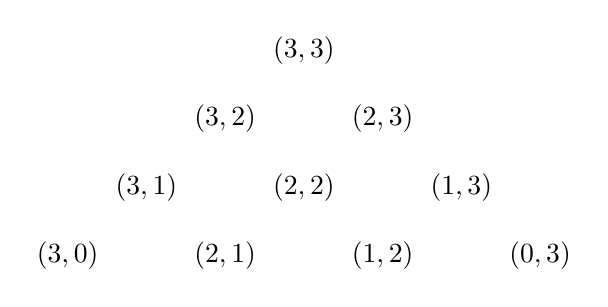
\begin{tikzpicture}[every node/.style={black}]
%	\coordinate (    ) at (Y+Z*2    , Y*1.7320508075    );
	\coordinate (e000) at (0+0*2, 0*0.86602540378);
	\coordinate (e001) at (1+0*2, 1*0.86602540378);
	\coordinate (e002) at (0+1*2, 0*0.86602540378);
	\coordinate (e011) at (2+0*2, 2*0.86602540378);
	\coordinate (e012) at (1+1*2, 1*0.86602540378);
	\coordinate (e022) at (0+2*2, 0*0.86602540378);
	\coordinate (e112) at (2+1*2, 2*0.86602540378);
	\coordinate (e122) at (1+2*2, 1*0.86602540378);
	\coordinate (e222) at (0+3*2, 0*0.86602540378);
	\coordinate (e111) at (3+0*2, 3*0.86602540378);

	\filldraw (e000) node{$(3,0)$};
	\filldraw (e001) node{$(3,1)$};
	\filldraw (e011) node{$(3,2)$};
	\filldraw (e002) node{$(2,1)$};
	\filldraw (e012) node{$(2,2)$};
	\filldraw (e111) node{$(3,3)$};
	\filldraw (e022) node{$(1,2)$};
	\filldraw (e112) node{$(2,3)$};
	\filldraw (e122) node{$(1,3)$};
	\filldraw (e222) node{$(0,3)$};
\end{tikzpicture}
\end{center}
The group action can be parameterized as:
\[\begin{aligned}
	(f\cdot a)(n,m) =& \sum_{(n',m')\preceq (n,m)}f(n',m')a[(n',m'),(n,m)]\\
	=& \sum_{k=N}^{n+m}\sum_{l=k-n}^{m}f(k-l,l)a[(k-l,l),(n,m)]\\
\end{aligned}\]
When we define the function on intervals as:
\[a[(k-l,l),(n,m)] = (1-\lambda)^{m-l}\lambda^{n-k+l}\binom{n+m-k}{n-k+l}\]
And the function $f(n,m)$ as some points in $\mathbb{R}^p$ then $(f\cdot a)(n,m)$ is the sum of Bézier curves controled the points preceding $(n,m)$ at $\lambda$.

\subsubsection{Example:}
Let $N=3$, the range of $f$ be $\mathbb{R}^2$, and $f(n,m)$ be no-zero only when $n+m=3$.
This situation may be graphically represented as:
\begin{center}
\begin{tikzpicture}[every node/.style={black}]
%	\coordinate (    ) at (Y+Z*2    , Y*1.7320508075    );
	\coordinate (e000) at (0+0*2, 0*0.86602540378);
	\coordinate (e001) at (1+0*2, 1*0.86602540378);
	\coordinate (e002) at (0+1*2, 0*0.86602540378);
	\coordinate (e011) at (2+0*2, 2*0.86602540378);
	\coordinate (e012) at (1+1*2, 1*0.86602540378);
	\coordinate (e022) at (0+2*2, 0*0.86602540378);
	\coordinate (e112) at (2+1*2, 2*0.86602540378);
	\coordinate (e122) at (1+2*2, 1*0.86602540378);
	\coordinate (e222) at (0+3*2, 0*0.86602540378);
	\coordinate (e111) at (3+0*2, 3*0.86602540378);

	\filldraw (e000) node{$P_0$};
	\filldraw (e001) node{$0$};
	\filldraw (e011) node{$0$};
	\filldraw (e002) node{$P_1$};
	\filldraw (e012) node{$0$};
	\filldraw (e111) node{$0$};
	\filldraw (e022) node{$P_2$};
	\filldraw (e112) node{$0$};
	\filldraw (e122) node{$0$};
	\filldraw (e222) node{$P_3$};
\end{tikzpicture}
\end{center}
A similar, but more crowded, representation of $f\cdot a$ is given by:
\begin{center}
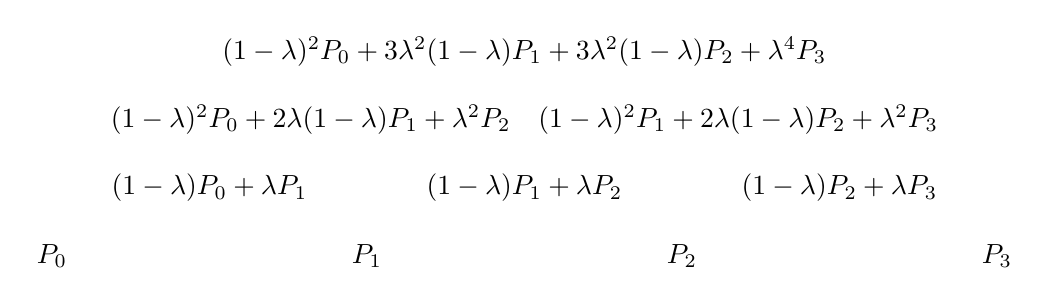
\begin{tikzpicture}[every node/.style={black}]
%	\coordinate (    ) at (Y+Z*2    , Y*1.7320508075    );
	\coordinate (e000) at (2*0+0*4, 0*0.86602540378);
	\coordinate (e001) at (2*1+0*4, 1*0.86602540378);
	\coordinate (e002) at (2*0+1*4, 0*0.86602540378);
	\coordinate (e011) at (2*2+0*4, 2*0.86602540378);
	\coordinate (e012) at (2*1+1*4, 1*0.86602540378);
	\coordinate (e022) at (2*0+2*4, 0*0.86602540378);
	\coordinate (e112) at (2*2+1*4, 2*0.86602540378);
	\coordinate (e122) at (2*1+2*4, 1*0.86602540378);
	\coordinate (e222) at (2*0+3*4, 0*0.86602540378);
	\coordinate (e111) at (2*3+0*4, 3*0.86602540378);


	\filldraw (e000) node{$P_0$};
	\filldraw (e001) node{$(1-\lambda) P_0+\lambda P_1$};
	\filldraw (e002) node{$P_1$};
	\filldraw (e012) node{$(1-\lambda) P_1+\lambda P_2$};
	\filldraw (e111) node{$(1-\lambda)^2P_0+3\lambda^2(1-\lambda) P_1+3\lambda^2(1-\lambda) P_2+\lambda^4P_3$};
	\filldraw (e022) node{$P_2$};
	\filldraw (e122) node{$(1-\lambda)P_2+\lambda P_3$};
	\filldraw (e222) node{$P_3$};

	\path (e011) -- (e112) node[midway]{$(1-\lambda)^2P_0+2\lambda(1-\lambda) P_1+\lambda^2 P_2\quad(1-\lambda)^2P_1+2\lambda(1-\lambda) P_2+\lambda^2 P_3$};
\end{tikzpicture}
\end{center}
The Bézier Curves can be visually observed.

%\subsection{Hasse Diagram}
%\subsection{Change summation order?}
% Expand group action?
%\subsection{Invertability}
%recurisive with $\mu$
